\documentclass[a4paper]{article}\usepackage[]{graphicx}\usepackage[]{color}
%% maxwidth is the original width if it is less than linewidth
%% otherwise use linewidth (to make sure the graphics do not exceed the margin)
\makeatletter
\def\maxwidth{ %
  \ifdim\Gin@nat@width>\linewidth
    \linewidth
  \else
    \Gin@nat@width
  \fi
}
\makeatother

\definecolor{fgcolor}{rgb}{0.345, 0.345, 0.345}
\newcommand{\hlnum}[1]{\textcolor[rgb]{0.686,0.059,0.569}{#1}}%
\newcommand{\hlstr}[1]{\textcolor[rgb]{0.192,0.494,0.8}{#1}}%
\newcommand{\hlcom}[1]{\textcolor[rgb]{0.678,0.584,0.686}{\textit{#1}}}%
\newcommand{\hlopt}[1]{\textcolor[rgb]{0,0,0}{#1}}%
\newcommand{\hlstd}[1]{\textcolor[rgb]{0.345,0.345,0.345}{#1}}%
\newcommand{\hlkwa}[1]{\textcolor[rgb]{0.161,0.373,0.58}{\textbf{#1}}}%
\newcommand{\hlkwb}[1]{\textcolor[rgb]{0.69,0.353,0.396}{#1}}%
\newcommand{\hlkwc}[1]{\textcolor[rgb]{0.333,0.667,0.333}{#1}}%
\newcommand{\hlkwd}[1]{\textcolor[rgb]{0.737,0.353,0.396}{\textbf{#1}}}%
\let\hlipl\hlkwb

\usepackage{framed}
\makeatletter
\newenvironment{kframe}{%
 \def\at@end@of@kframe{}%
 \ifinner\ifhmode%
  \def\at@end@of@kframe{\end{minipage}}%
  \begin{minipage}{\columnwidth}%
 \fi\fi%
 \def\FrameCommand##1{\hskip\@totalleftmargin \hskip-\fboxsep
 \colorbox{shadecolor}{##1}\hskip-\fboxsep
     % There is no \\@totalrightmargin, so:
     \hskip-\linewidth \hskip-\@totalleftmargin \hskip\columnwidth}%
 \MakeFramed {\advance\hsize-\width
   \@totalleftmargin\z@ \linewidth\hsize
   \@setminipage}}%
 {\par\unskip\endMakeFramed%
 \at@end@of@kframe}
\makeatother

\definecolor{shadecolor}{rgb}{.97, .97, .97}
\definecolor{messagecolor}{rgb}{0, 0, 0}
\definecolor{warningcolor}{rgb}{1, 0, 1}
\definecolor{errorcolor}{rgb}{1, 0, 0}
\newenvironment{knitrout}{}{} % an empty environment to be redefined in TeX

\usepackage{alltt}
\usepackage{a4wide}
\usepackage[margin=.8in]{geometry}
\usepackage{colortbl}

\title{Comparison of Versions of Kinship Links}
\author{Joe Rodger's BG Team}
\IfFileExists{upquote.sty}{\usepackage{upquote}}{}
\begin{document}

\maketitle

\definecolor{goodColor}{rgb}{.9,1,.85}
\definecolor{sosoColor}{rgb}{1,0.9215686,0.6117647}
\definecolor{badColor}{rgb}{1,.85,.85}
\definecolor{nullColor}{rgb}{.9, 0.85, 0.95} %0.8000000 0.7529412 0.8549020
\setlength{\parindent}{0pt}%http://tex.stackexchange.com/questions/49188/how-to-insert-vertical-space-between-paragraphs

% Working directory: getwd();



% Working directory: getwd();
















% \textbf{RelationshipPaths Considered}: includedRelationshipPaths;\\
\textbf{Newer Links Version}: 1;
\textbf{Older Links Version}: 1;

\begin{knitrout}
\definecolor{shadecolor}{rgb}{0.969, 0.969, 0.969}\color{fgcolor}\begin{kframe}
\begin{verbatim}
Newer Links: naive roster
Older Links: naive roster
\end{verbatim}
\end{kframe}
\end{knitrout}

\begin{knitrout}
\definecolor{shadecolor}{rgb}{0.969, 0.969, 0.969}\color{fgcolor}
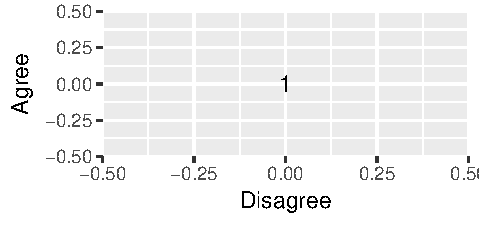
\includegraphics[width=\maxwidth]{figure/graph-roc-1} 

\end{knitrout}


% latex table generated in R 3.4.3 by xtable 1.8-2 package
% Tue Feb 13 16:10:08 2018
\begin{table}[ht]
\centering
\begingroup\large
\begin{tabular}{lrrrrr}
  \hline
R & Implicit2004 & Implicit & Roster & Explicit & Eventual \\ 
  \hline
0 & - & - & 174 & - & 1376 \\ 
  0.25 & - & - & 126 & - & 126 \\ 
  0.5 & - & - & 1017 & - & 1017 \\ 
  - &   0 & 2519 & 1202 & 2519 &   0 \\ 
   \hline
\end{tabular}
\endgroup
\caption{Counts for 97 Housemates} 
\end{table}
% latex table generated in R 3.4.3 by xtable 1.8-2 package
% Tue Feb 13 16:10:09 2018
\begin{table}[ht]
\centering
\begingroup\large
\begin{tabular}{lrrrrr}
  \hline
R & Implicit2004 & Implicit & Roster & Explicit & Eventual \\ 
  \hline
0 & - & - & 174 & - & 1376 \\ 
  0.25 & - & - & 126 & - & 126 \\ 
  0.5 & - & - & 1017 & - & 1017 \\ 
  - &   0 & 2519 & 1202 & 2519 &   0 \\ 
   \hline
\end{tabular}
\endgroup
\caption{Counts for 97 Housemates (Previous version of links)} 
\end{table}



% latex table generated in R 3.4.3 by xtable 1.8-2 package
% Tue Feb 13 16:10:09 2018
\begin{table}[ht]
\centering
\begin{tabular}{rrrrr}
  \hline
Count & RImplicit & RExplicit & RRoster & Delta \\ 
  \rowcolor{nullColor}  \hline
1202 & - & - & - & 0 \\ 
   \rowcolor{nullColor} 1017 & - & - & 0.500 & 0 \\ 
   \rowcolor{nullColor} 174 & - & - & 0.000 & 0 \\ 
   \rowcolor{nullColor} 126 & - & - & 0.250 & 0 \\ 
   \hline
\end{tabular}
\caption{Joint Frequencies for 97 Housemates} 
\end{table}



\end{document}
